\chapter{Results}\label{ch:results}

During the execution of the network, a number of plots have been made in order to visualize any outliers, along with a list of any anomalies the network has found. Keep in mind that these plots and anomalies are all based on 5\% of the authentication data.

\begin{figure}
	\begin{center}
		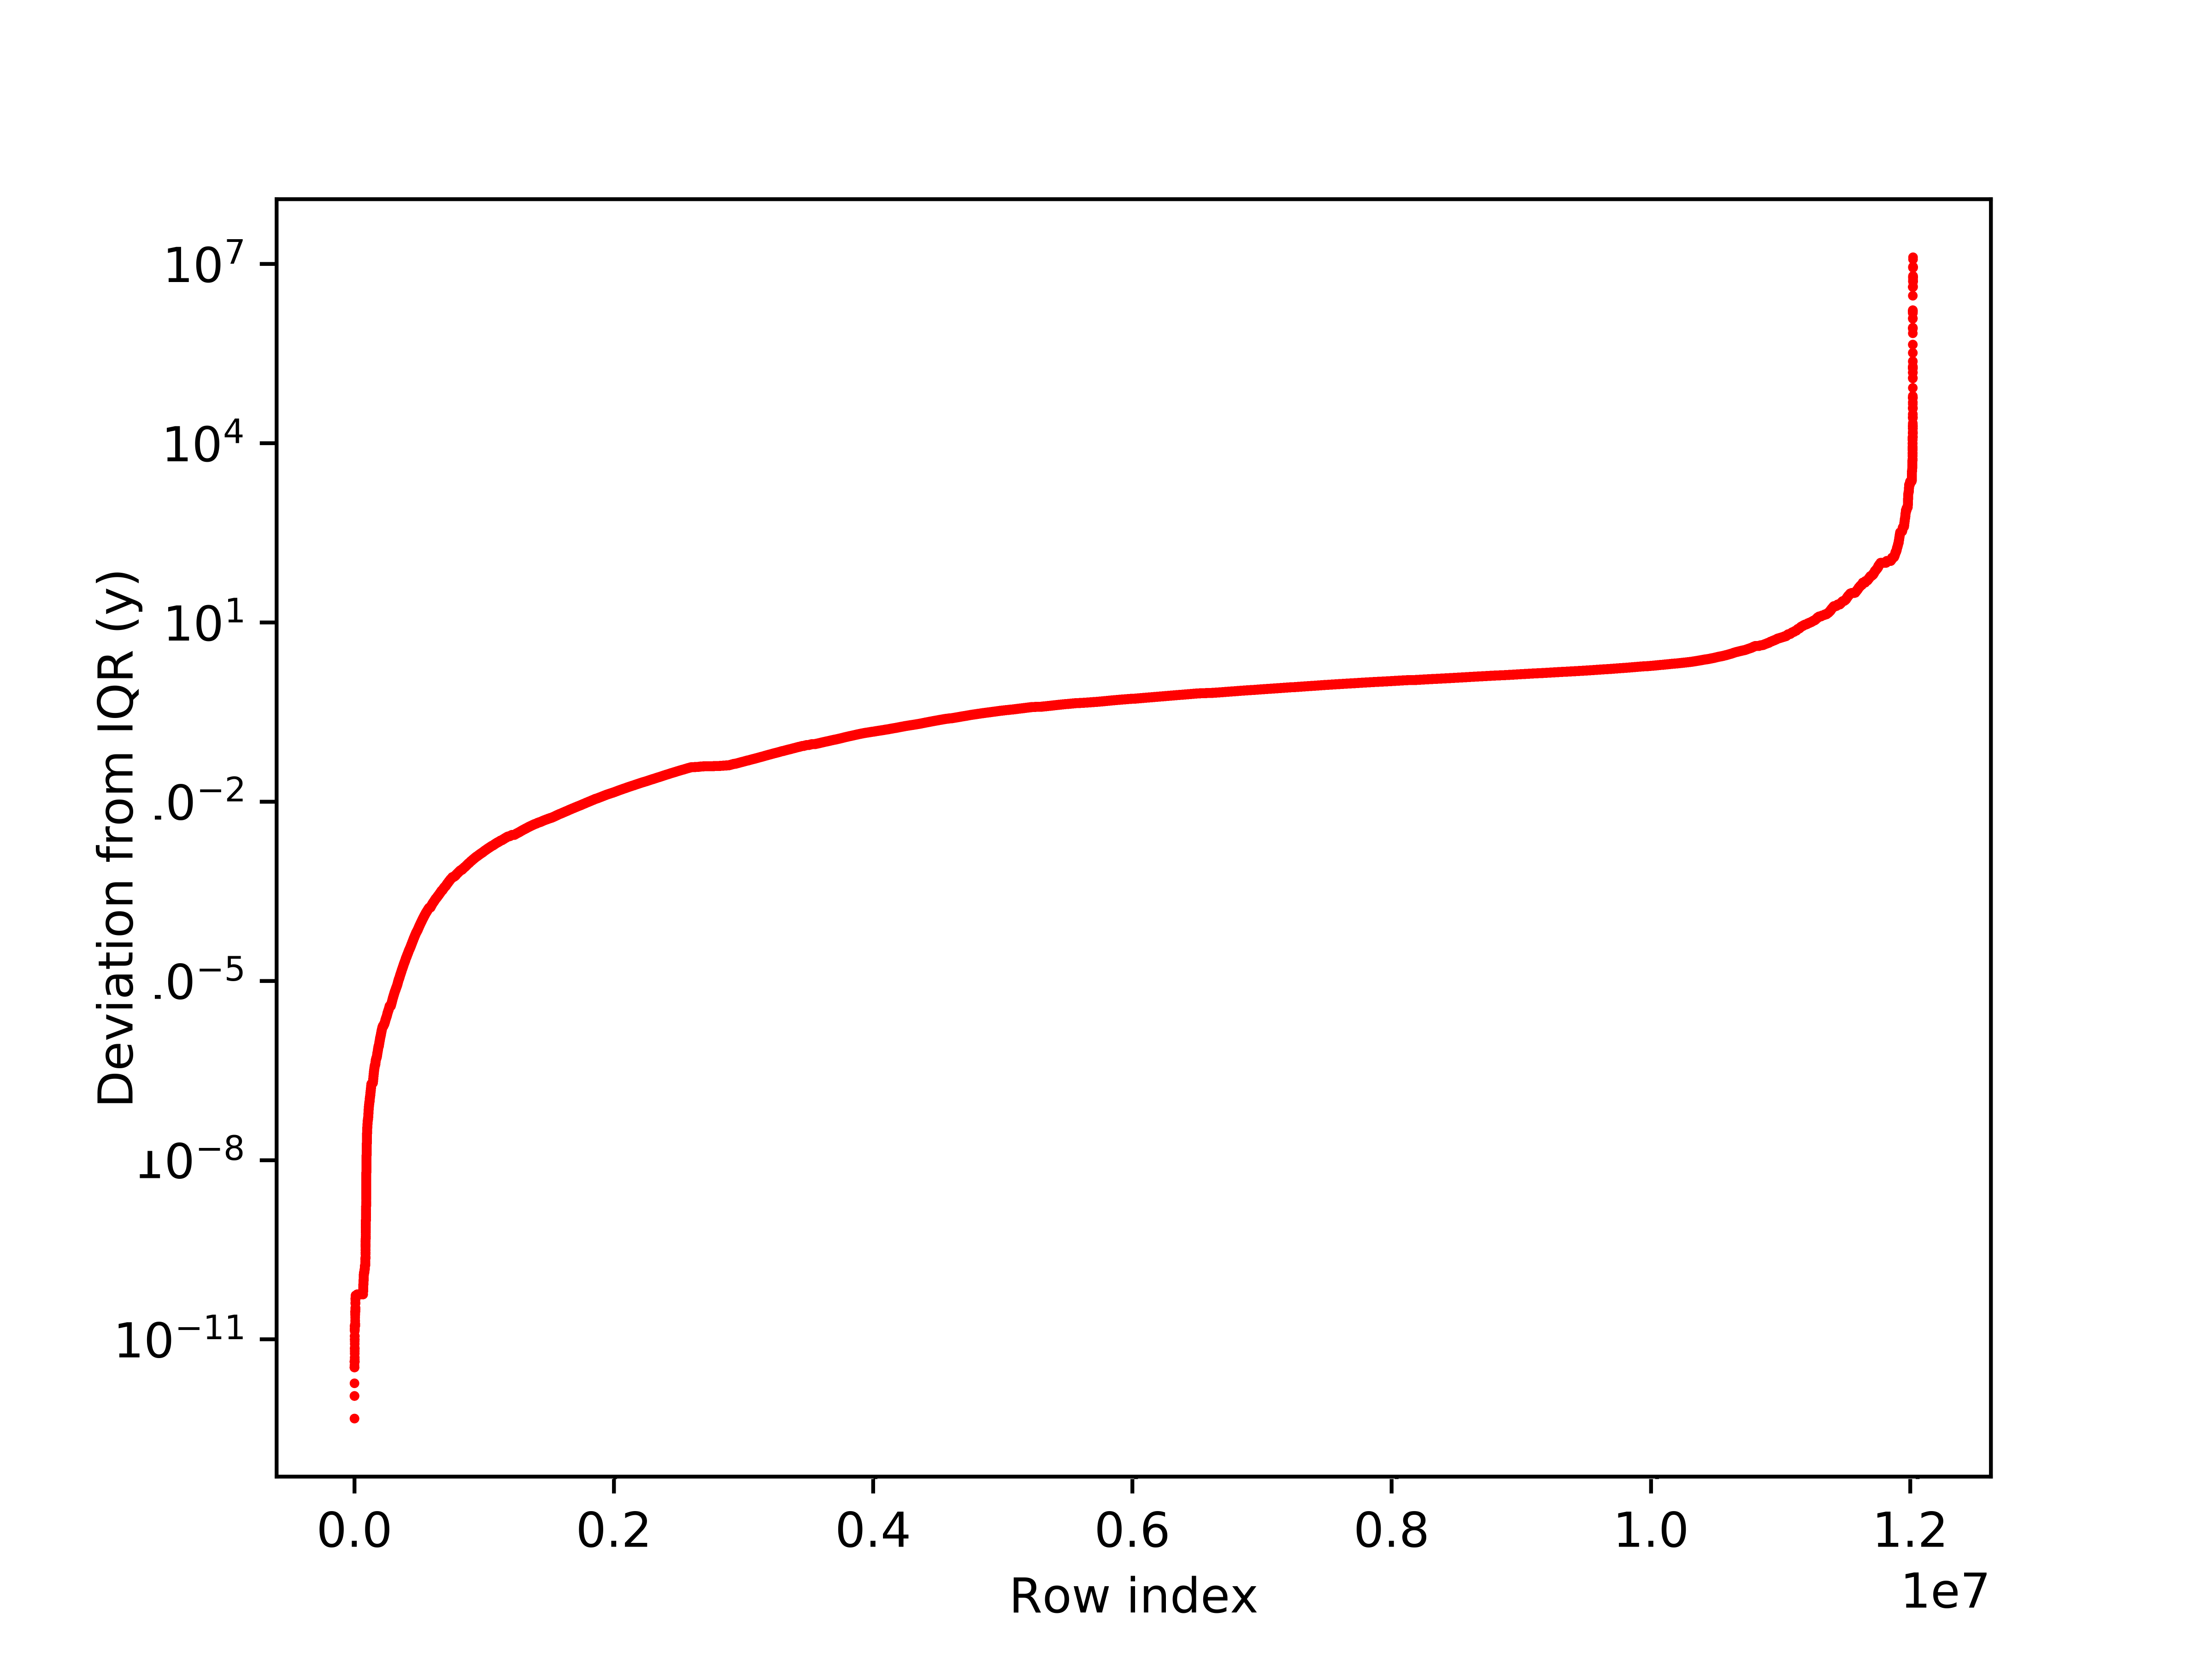
\includegraphics[scale=0.1]{results/all_deviations}
	\end{center}
	\caption{All deviations (\(y\)) from the IQR.~\label{fig:iqr_scale}}
\end{figure}

In order to get an idea of how much an action deviates relative to its containing distribution, a function has been created with which this can be calculated. In the function indicating the max value of \(x\) before \(x\) becomes an outlier, replacing 1.5 with \(y\) gives an indication of this deviation from its containing distribution. This gives the following function:

$$ x > Q3 + y IQR $$

In order to find \(y\) here, the following function is used:

$$ y = (x - Q3) / IQR $$

This \(y\) value is then plotted, the result of which can be seen in figure~\ref{fig:iqr_scale}. As can be seen in the figure, there are quite a number of outliers, some of which having outliers that fall far beyond the cutoff value of 1.5. From this, we can conclude that at least some anomalies are being found. 

\begin{figure}
	\begin{center}
		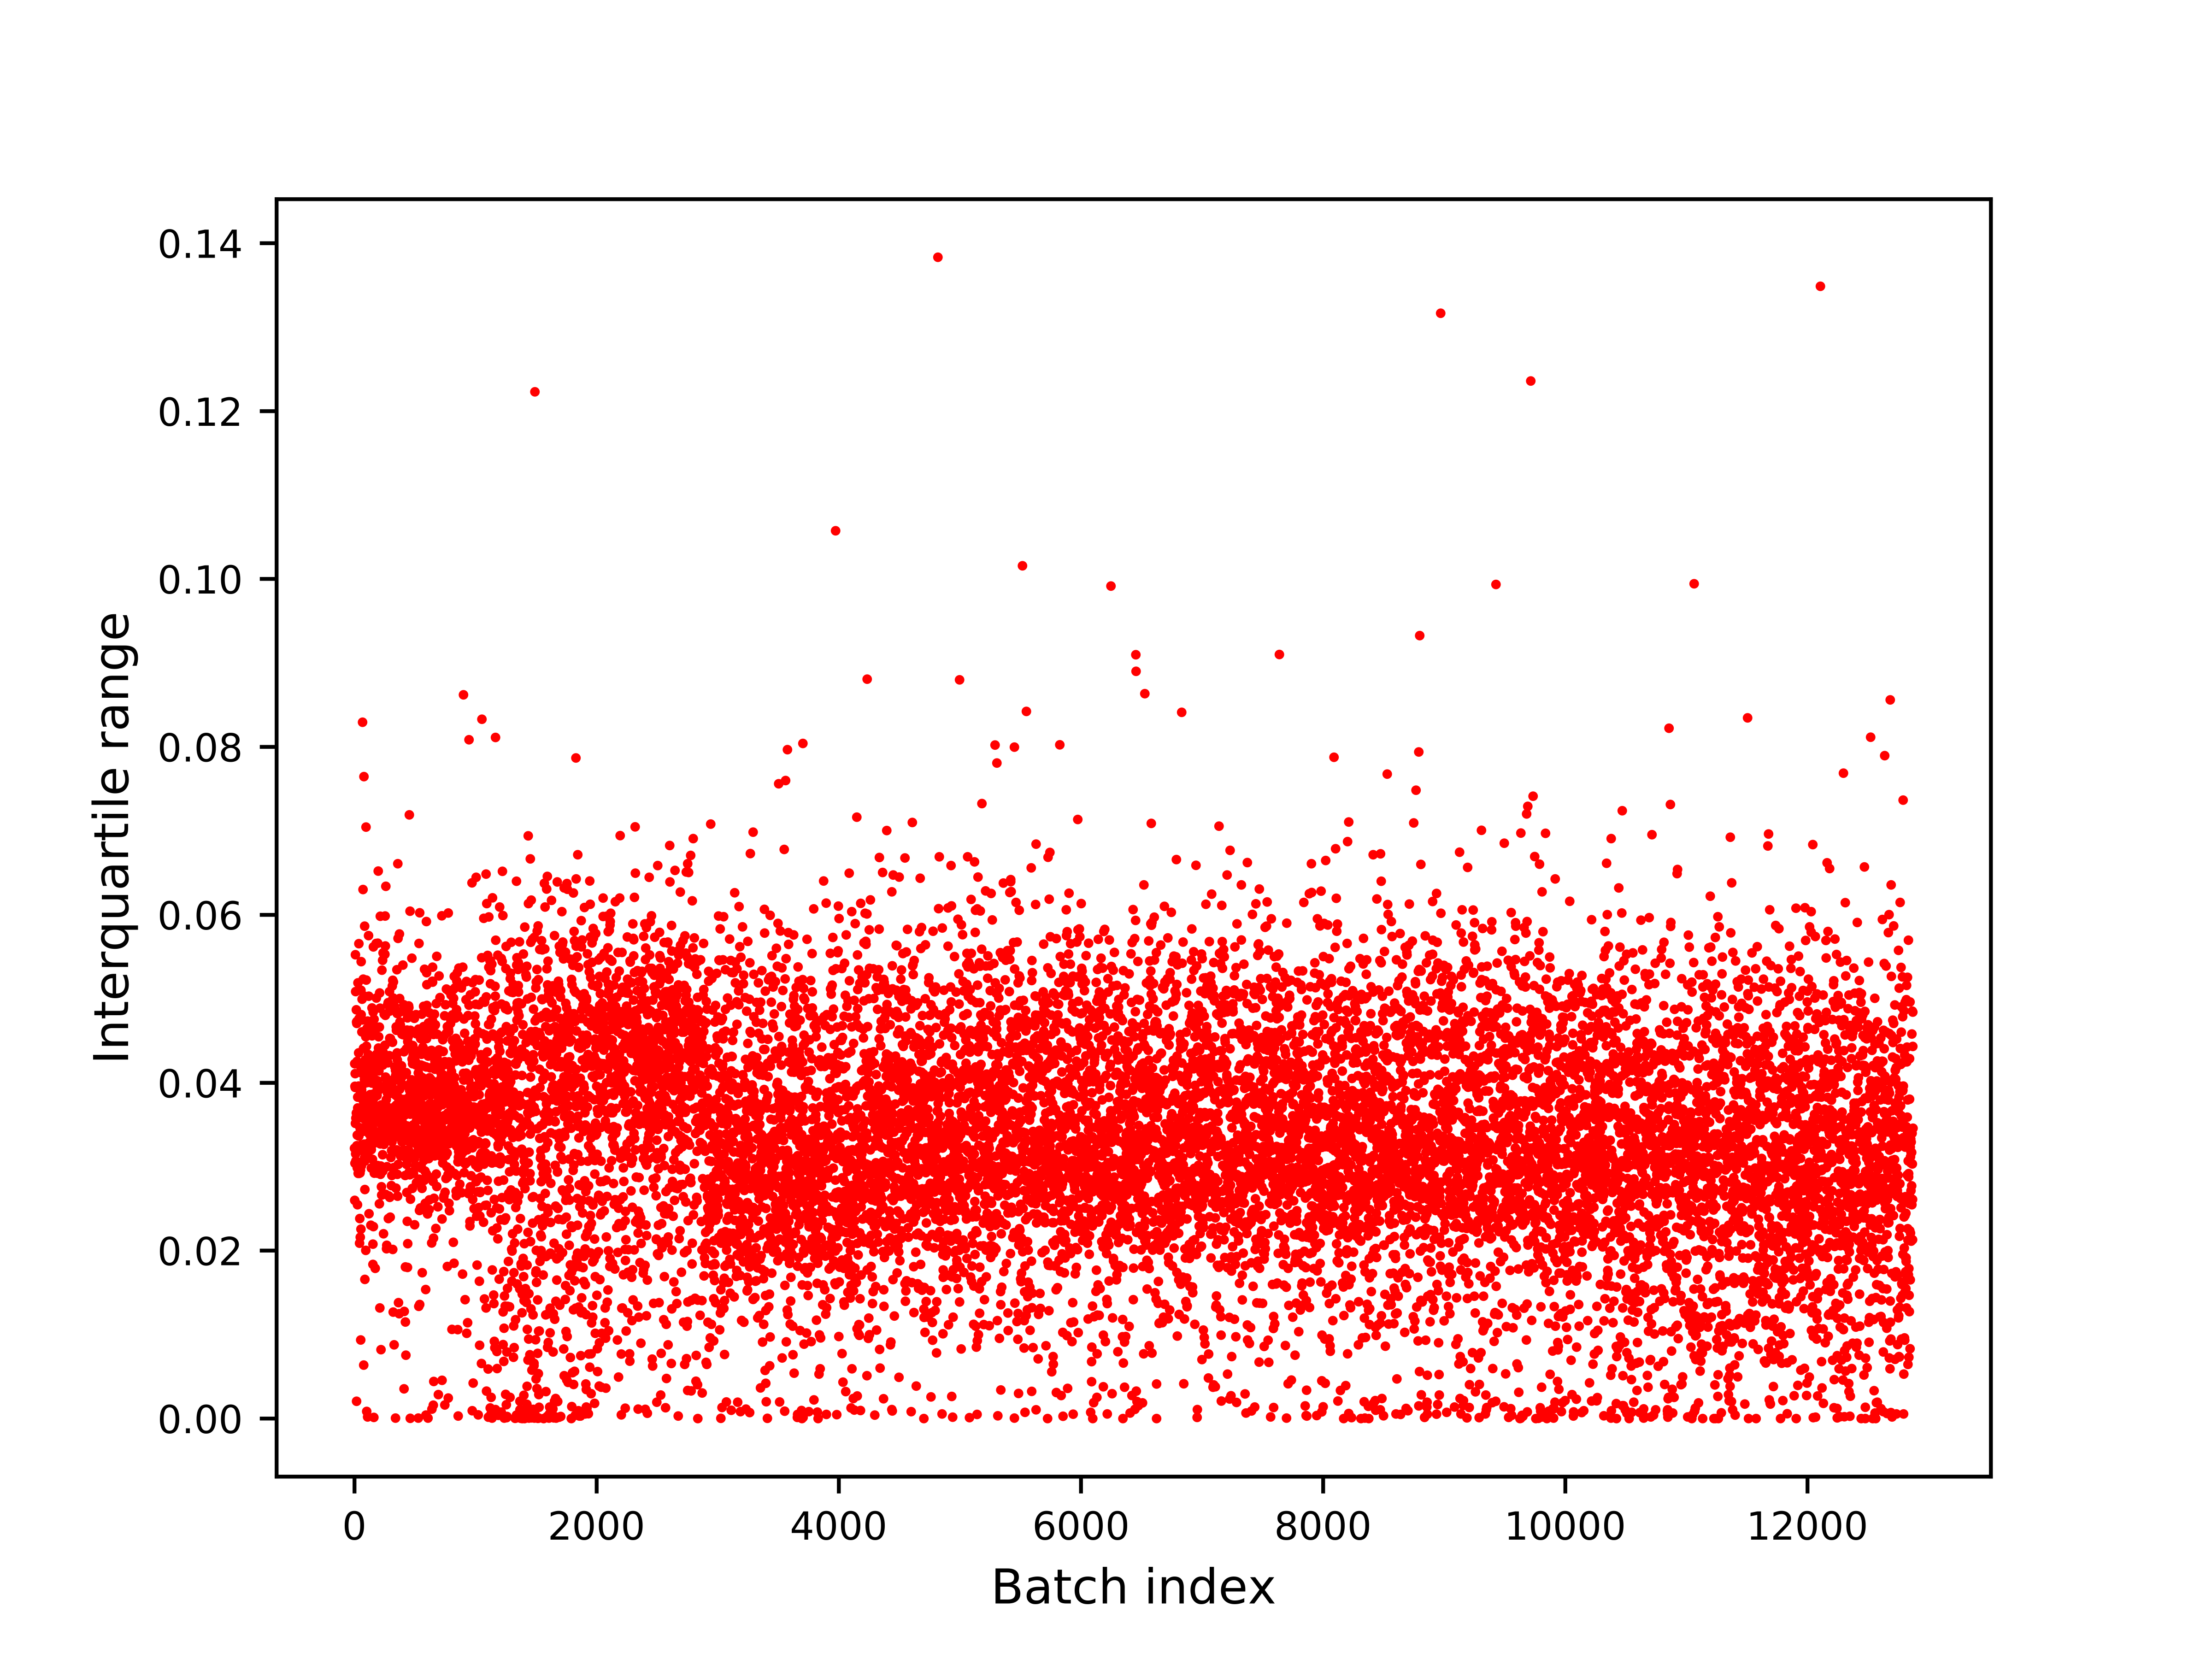
\includegraphics[scale=1.6]{results/iqrs}
	\end{center}
	\caption{All IQR values.~\label{fig:iqrs}}
\end{figure}

As can be seen in figure~\ref{fig:iqrs}, the IQRs tend to be fairly close to each other, meaning the mean losses are close to each other as well. This shows that the network is relatively successful at modeling user behavior, as the difference between the expected and actual action calculated by the loss function shows few big spikes. A network that is unsuccessful at this would have inconsistent IQRs as the losses would fluctuate more from user to user and would show higher values indicating bad predictions.

\begin{figure}
	\begin{center}
		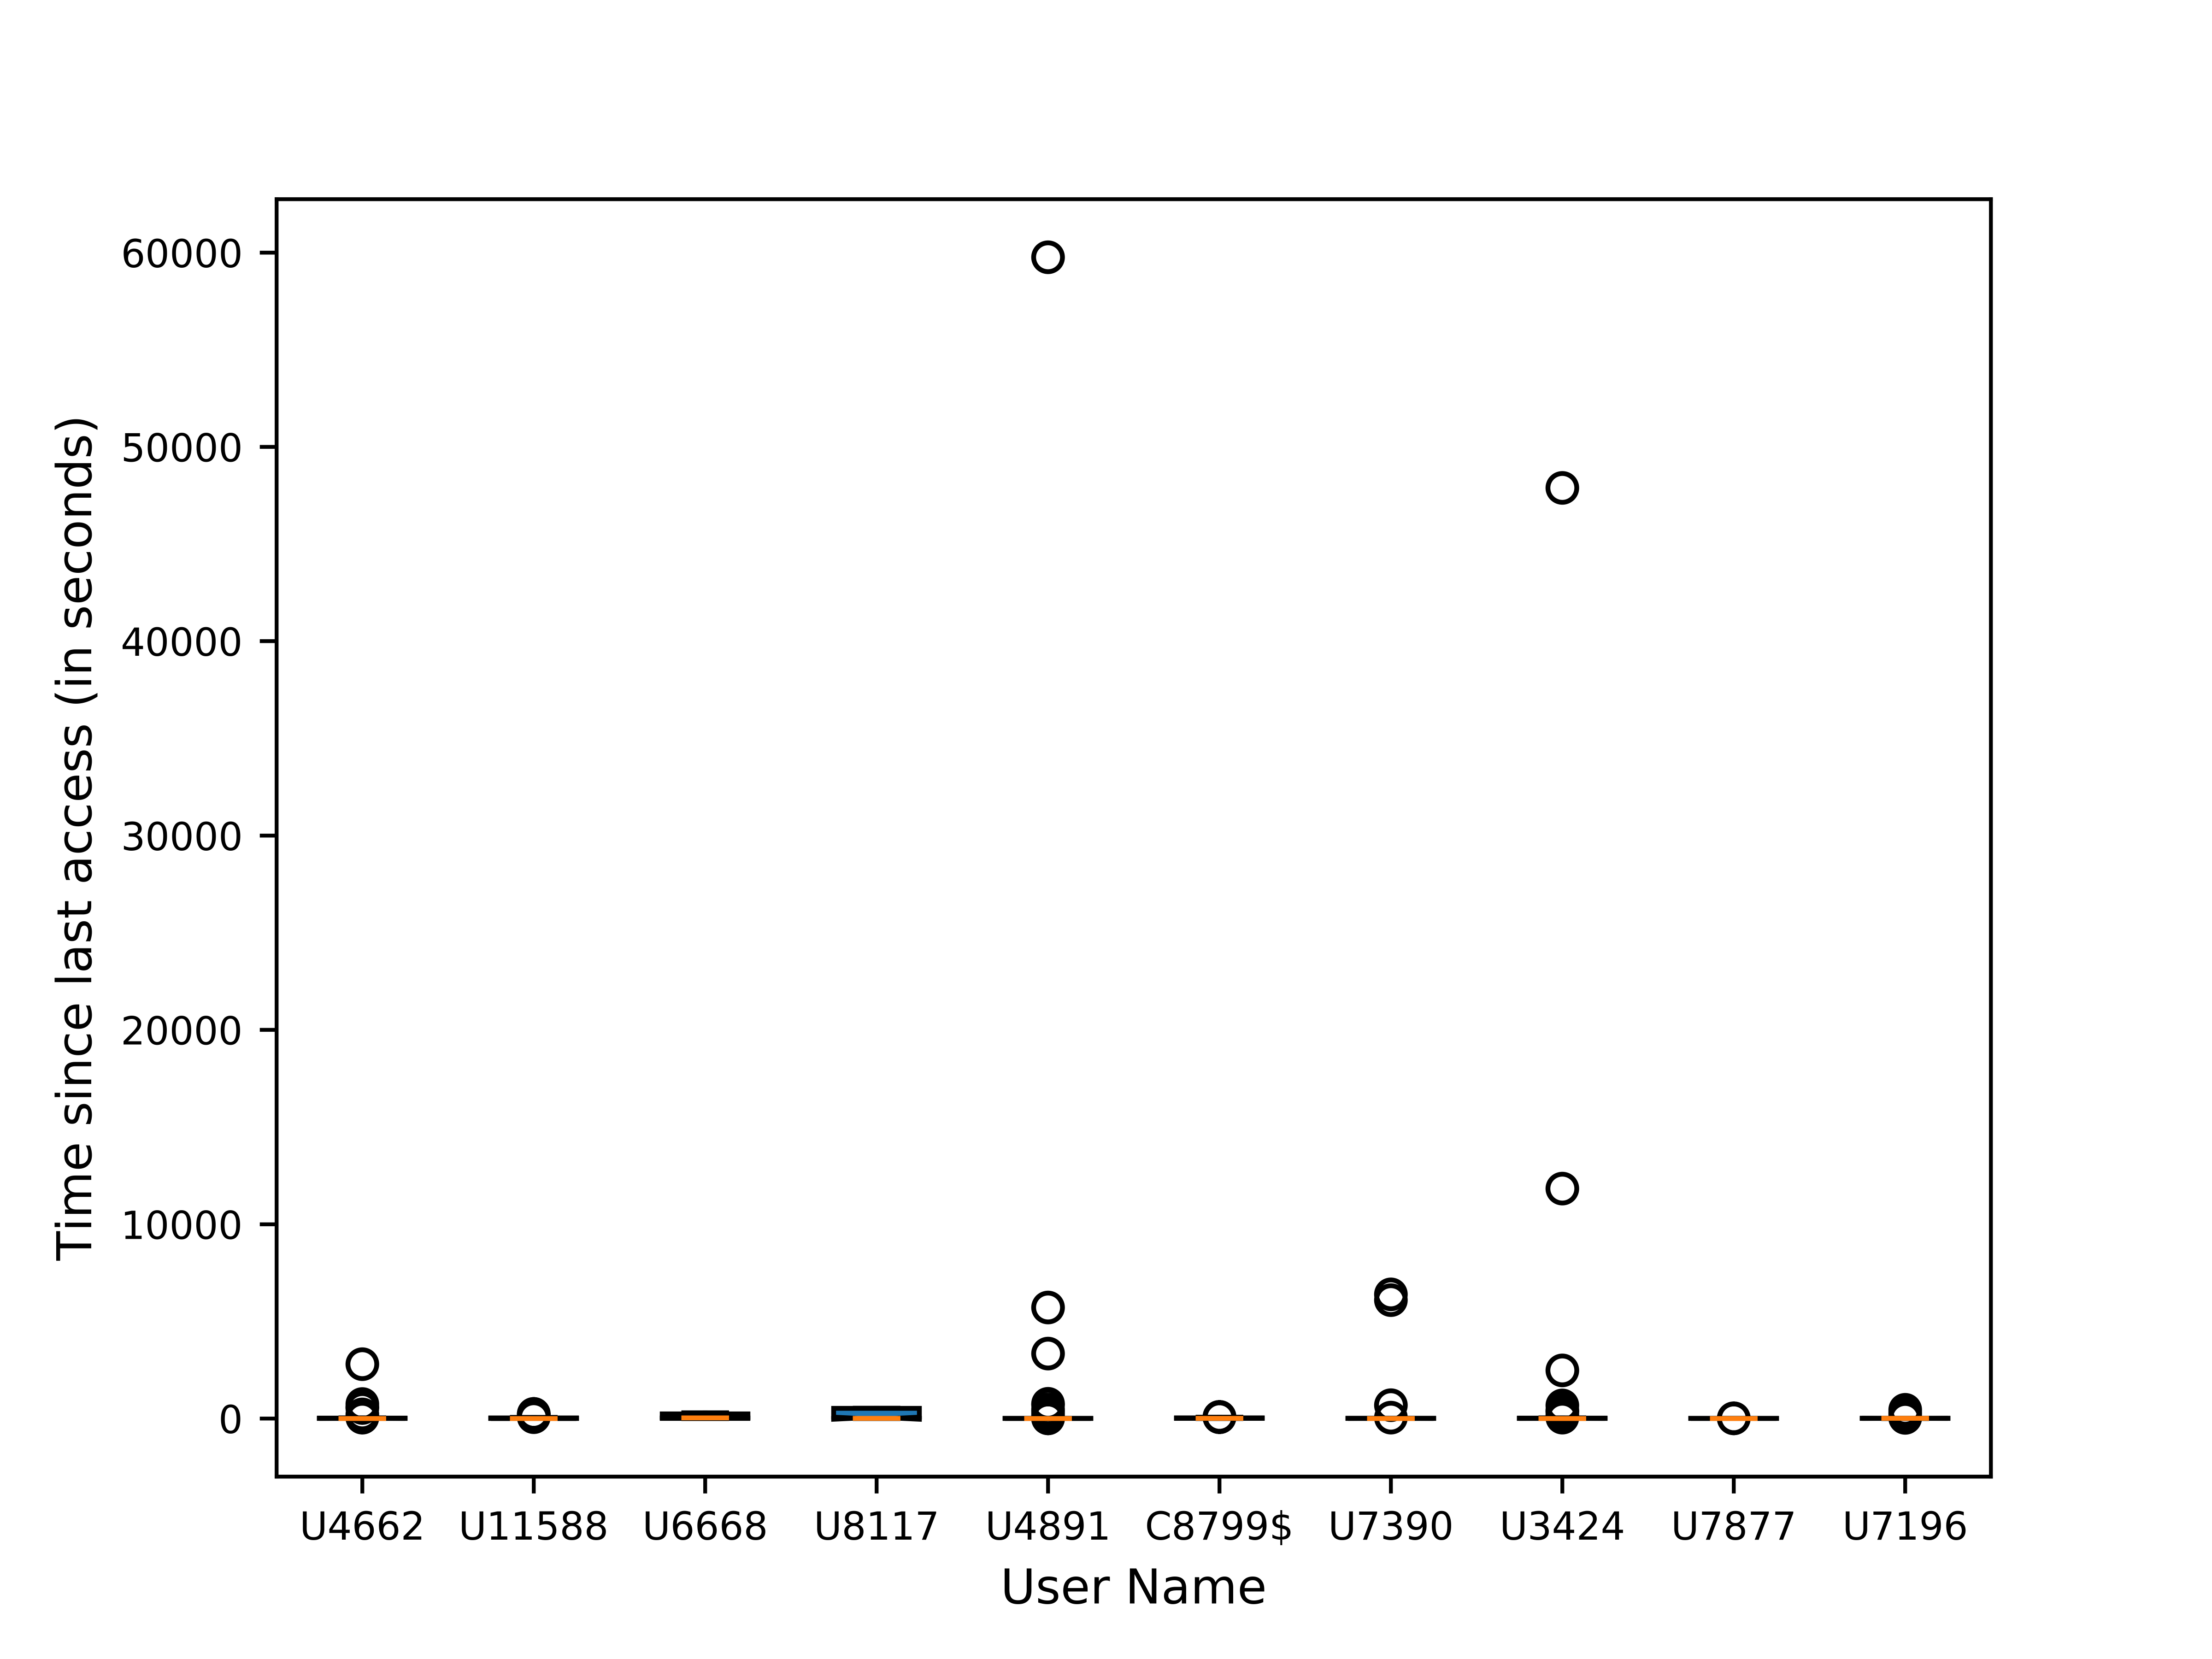
\includegraphics[scale=1.6]{results/highest_offender_time_since_last_access}
	\end{center}
	\caption{The top 10 highest offenders' seconds since last access.~\label{fig:time_since_last_access}}
\end{figure}

Focussing on the highest offending users allows us to see more clearly why the network thought certain users were deemed anomalies and whether the network may have been right.

In figure~\ref{fig:time_since_last_access} we take a closer look at the time since the last network access for the top 10 highest offending users. This clearly shows some very big deviations from users' times since their last network access. For example, U4891 consistently has a very low time since last access, as can be seen from the box plot being very small and concentrated around that area. However, there are some small and bigger deviations from this average, probably causing the network to flag them as suspicious.

\begin{table}[htbp]
	\centering
	\caption{The predicted features vs the actual features of the top offender (precision set to 2 decimals)}\label{tab:predicted_vs_actual_top}
	\begin{tabular}{lll}
		Label & Actual & Predicted \\ \midrule
		time\_since\_last\_access & 0 & 0.00 \\
		domains\_delta & 0 & 0.00 \\
		dest\_users\_delta & 0 & 0.00 \\
		src\_computers\_delta & 0 & 0.00 \\
		dest\_computers\_delta & 0 & 0.00 \\
		percentage\_failed\_logins & 0.0 & 0.00 \\
		success\_failure & 1 & 0.4 \\
		auth\_type\_0 & 1 & 0.1 \\
		auth\_type\_1 & 0 & 0.19 \\
		auth\_type\_2 & 0 & 0.00 \\
		auth\_type\_3 & 0 & 0.00 \\
		auth\_type\_4 & 0 & 0.00 \\
		auth\_type\_5 & 0 & 0.00 \\
		auth\_type\_6 & 0 & 0.00 \\
		auth\_type\_7 & 0 & 0.00 \\
		auth\_type\_8 & 0 & 0.00 \\
		auth\_type\_9 & 0 & 0.69 \\
		auth\_type\_10 & 0 & 0.01 \\
		logon\_type\_0 & 0 & 0.02 \\
		logon\_type\_1 & 0 & 0.00 \\
		logon\_type\_2 & 0 & 0.00 \\
		logon\_type\_3 & 0 & 0.00 \\
		logon\_type\_4 & 1 & 0.00 \\
		logon\_type\_5 & 0 & 0.05 \\
		logon\_type\_6 & 0 & 0.08 \\
		logon\_type\_7 & 0 & 0.08 \\
		logon\_type\_8 & 0 & 0.08 \\
		auth\_orientation\_0 & 0 & 0.58 \\
		auth\_orientation\_1 & 0 & 0.06 \\
		auth\_orientation\_2 & 0 & 0.00 \\
		auth\_orientation\_3 & 0 & 0.01 \\
		auth\_orientation\_4 & 0 & 0.00 \\
		auth\_orientation\_5 & 1 & 0.28
	\end{tabular}
\end{table}

\begin{table}[htbp]
	\centering
	\caption{The highest offending user's previous logins before the anomaly}\label{tab:prev_logins}
	\resizebox{\linewidth}{!}{
		\begin{tabular}{lllllllll}
			time & source user@domain & destination user@domain & source computer & destination computer & authentication type & logon type & authentication orientation & success/failure \\ \midrule
			212020000 & C14012\$@DOM1 & C14012\$@DOM1 & C14012 & C2106 & Network & LogOn & Success \\
			212020000 & C14012\$@DOM1 & C14012\$@DOM1 & C14012 & C2106 & Network & LogOn & Success \\
			212020000 & C14012\$@DOM1 & C14012\$@DOM1 & C2106 & C2106 & Network & LogOff & Success \\
			212023000 & C14012\$@DOM1 & C14012\$@DOM1 & C2106 & C2106 & Network & LogOff & Success \\
			212029000 & C14012\$@DOM1 & C14012\$@DOM1 & C2106 & C2106 & Network & LogOff & Success \\
			212043000 & C14012\$@DOM1 & C14012\$@DOM1 & C457 & C457 & Network & LogOff & Success \\
			212758000 & C14012\$@DOM1 & C14012\$@DOM1 & C14012 & C457 & Network & LogOn & Success \\
			212772000 & C14012\$@DOM1 & C14012\$@DOM1 & C457 & C457 & Network & LogOff & Success \\
			212784000 & C14012\$@DOM1 & C14012\$@DOM1 & C14012 & C457 & Network & LogOn & Success \\
			212797000 & C14012\$@DOM1 & C14012\$@DOM1 & C457 & C457 & Network & LogOff & Success \\
			213233000 & C14012\$@DOM1 & U6147@DOM1 & C14012 & C14012 & Unlock & LogOn & Success \\
			213233000 & C14012\$@DOM1 & U6147@DOM1 & C1521 & C14012 & Unlock & LogOn & Success \\
			213657000 & C14012\$@DOM1 & C14012\$@DOM1 & C14012 & C457 & Network & LogOn & Success \\
			213671000 & C14012\$@DOM1 & C14012\$@DOM1 & C457 & C457 & Network & LogOff & Success \\
			213698000 & C14012\$@DOM1 & C14012\$@DOM1 & C14012 & C457 & Network & LogOn & Success \\
			213707000 & C14012\$@DOM1 & C14012\$@DOM1 & C457 & C457 & Network & LogOff & Success \\
			214557000 & C14012\$@DOM1 & C14012\$@DOM1 & C14012 & C457 & Network & LogOn & Success \\
			214571000 & C14012\$@DOM1 & C14012\$@DOM1 & C457 & C457 & Network & LogOff & Success \\
			214598000 & C14012\$@DOM1 & C14012\$@DOM1 & C14012 & C457 & Network & LogOn & Success \\
			214608000 & C14012\$@DOM1 & C14012\$@DOM1 & C457 & C457 & Network & LogOff & Success \\
			215457000 & C14012\$@DOM1 & C14012\$@DOM1 & C14012 & C457 & Network & LogOn & Success \\
			215471000 & C14012\$@DOM1 & C14012\$@DOM1 & C457 & C457 & Network & LogOff & Success \\
			215524000 & C14012\$@DOM1 & C14012\$@DOM1 & C14012 & C457 & Network & LogOn & Success \\
			215533000 & C14012\$@DOM1 & C14012\$@DOM1 & C457 & C457 & Network & LogOff & Success \\
			216357000 & C14012\$@DOM1 & C14012\$@DOM1 & C14012 & C457 & Network & LogOn & Success \\
			216371000 & C14012\$@DOM1 & C14012\$@DOM1 & C457 & C457 & Network & LogOff & Success \\
			216392000 & C14012\$@DOM1 & C14012\$@DOM1 & C14012 & C457 & Network & LogOn & Success \\
			216405000 & C14012\$@DOM1 & C14012\$@DOM1 & C457 & C457 & Network & LogOff & Success \\
			217145000 & C14012\$@DOM1 & C14012\$@DOM1 & C14012 & C2106 & Network & LogOn & Success \\
			217149000 & C14012\$@DOM1 & C14012\$@DOM1 & C2106 & C2106 & Network & LogOff & Success \\
			217257000 & C14012\$@DOM1 & C14012\$@DOM1 & C14012 & C457 & Network & LogOn & Success \\
			217271000 & C14012\$@DOM1 & C14012\$@DOM1 & C457 & C457 & Network & LogOff & Success
		\end{tabular}
	}
\end{table}

The highest offending action's predicted vs actual action are shown in Table~\ref{tab:predicted_vs_actual_top}. In this table (and following tables) features that are integers and not floats have been depicted as such, as all but the \(percentage\_failed\_logins\) features are integers. Any predictions made by the network are trimmed to 1 decimal point.

As can be seen, the action itself isn't very weird, simply using a different method of authentication, a different method of logging in and a different authentication orientation. These methods themselves are not inherently anomalies, but the network learned that these actions are rarely made by the user, assigning a value of 0.0 to \(logon\_type\_4\) (interactive logon) and a value of 0.0 to \(auth\_type\_0\) (NTLM). When compared to the user's previous logins in Table~\ref{tab:prev_logins}, the last action really stands out as different. Many anomalies like this have been found. The user often logs in after a really long time or significantly changes their behavior by logging in using methods rarely or never used before. This signals that the network is doing a good job at recognizing the user's behavior and finding anything that deviates from it.